\documentclass[10pt, aspectratio=169, handout]{beamer}
\usefonttheme{professionalfonts}

\mode<presentation>
{ 
  \usetheme{Berkeley}
  \usecolortheme{beaver}
  \usefonttheme{default}
  \setbeamertemplate{navigation symbols}{} 
  \setbeamertemplate{caption}[numbered]
} 

\setbeamertemplate{footline}{%
  \leavevmode%
  \hbox{% 
    \begin{beamercolorbox}[wd=.85\paperwidth,ht=2.5ex,dp=1ex,left]{author in head/foot}% 
      \usebeamerfont{author in head/foot}Digital Signal Processing, Fall 2025%
    \end{beamercolorbox}% 
    \begin{beamercolorbox}[wd=.15\paperwidth,ht=2.5ex,dp=1ex,right]{date in head/foot}% 
      \hspace*{0.5em}\insertframenumber{} / \inserttotalframenumber\hspace*{0.5em}% 
    \end{beamercolorbox}% 
  }%
  \vskip0pt%
}

\usepackage[english]{babel}
\usepackage[utf8x]{inputenc}
\usepackage{tikz}
\usepackage{pgfplots}
\usepackage{array}
\usepackage{makecell}
\usepackage{verbatim}
\usepackage{graphicx}
\usepackage{subcaption}
\usepackage{amsfonts}
\usepackage{amsmath}
\usepackage{bm}
\usepackage{epstopdf}
\captionsetup{compatibility=false}
\usepackage[absolute,overlay]{textpos}
\usetikzlibrary{calc}
\usetikzlibrary{pgfplots.fillbetween, backgrounds}
\usetikzlibrary{positioning}
\usetikzlibrary{pgfplots.groupplots}
\usetikzlibrary{plotmarks}
\usetikzlibrary{calc}
\usetikzlibrary{positioning,arrows.meta}
\usepgfplotslibrary{groupplots}
\pgfplotsset{compat=newest} 

\usepackage{hyperref}
\hypersetup{
    colorlinks=true,
    linkcolor=blue,
    filecolor=magenta,      
    urlcolor=cyan,
}

\title[ECEN 463/863]{Continuous-Time Processing of Discrete-Time Signals}
\author{Maxx Seminario}
\institute{University of Nebraska-Lincoln}
\date{Fall 2025}

\begin{document}

\begin{frame}
  \titlepage
\end{frame}

\section{Introduction}

\begin{frame}{Overview: System Architecture}
\small % slightly smaller text so the diagram fits comfortably
\textbf{Complementary to Previous Topic}:
\begin{itemize}
    \item Previously: Discrete-time processing of continuous-time signals
    \item Now: Continuous-time processing of discrete-time signals
\end{itemize}

\vspace{0.25cm}
\textbf{General System Configuration}:
\begin{center}
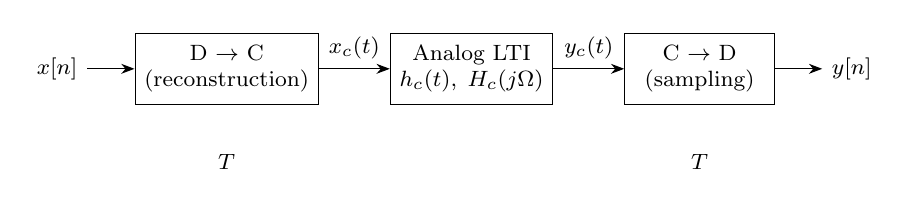
\begin{tikzpicture}[>=Stealth, node distance=0.6cm, auto, every node/.style={font=\footnotesize}]
  % moderate compact block style (not too tight)
  \tikzset{block/.style={draw, minimum width=1.9cm, minimum height=0.9cm, align=center}}
  % nodes with balanced spacing so the slide fits but isn't cramped
  \node (xn) {$x[n]$};
  \node[block, right=0.6cm of xn] (dac) {D $\to$ C\\(reconstruction)};
  \node[block, right=0.9cm of dac] (hc) {Analog LTI\\$h_c(t),\;H_c(j\Omega)$};
  \node[block, right=0.9cm of hc] (adc) {C $\to$ D\\(sampling)};
  \node (yn) [right=0.6cm of adc] {$y[n]$};

  % arrows with short, visible extensions (0.3cm)
  \draw[->] (xn.east) -- ++(0.25,0) -- (dac.west);
  % moved the continuous-time labels slightly to the right using xshift
  \draw[->] (dac.east) -- ++(0.3,0) node[midway, above, xshift=3mm] {$x_c(t)$} -- (hc.west);
  \draw[->] (hc.east) -- ++(0.3,0) node[midway, above, xshift=3mm] {$y_c(t)$} -- (adc.west);
  \draw[->] (adc.east) -- ++(0.25,0) -- (yn.west);

  % sampling period labels under the converters
  \node [below=0.5cm of dac] {$T$};
  \node [below=0.5cm of adc] {$T$};
\end{tikzpicture}
\end{center}

\vspace{0.25cm}
\textbf{Key Characteristics}:
\begin{itemize}
    \item Input and output: discrete-time sequences
    \item Intermediate processing: continuous-time domain
    \item Provides useful interpretation of certain discrete-time systems
    \item Not typically implemented
\end{itemize}
\end{frame}

\begin{frame}{Bandlimited Signal Constraint}
\textbf{Fundamental Property}:

The ideal D/C converter produces a bandlimited signal:
\[
X_c(j\Omega) = 0, \quad |\Omega| \geq \pi/T
\]

\vspace{0.3cm}
\textbf{Consequence}: No aliasing in C/D conversion
\begin{itemize}
    \item $y_c(t)$ is also bandlimited: $Y_c(j\Omega) = 0$ for $|\Omega| \geq \pi/T$
    \item Sampling $y_c(t)$ at rate $1/T$ satisfies Nyquist criterion
    \item Perfect reconstruction of $y[n]$ from $y_c(nT)$
\end{itemize}

\begin{center}
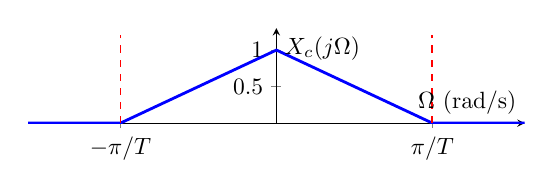
\begin{tikzpicture}[scale=0.85]
    \begin{axis}[
        width=9cm, height=3cm,
        xlabel={$\Omega$ (rad/s)},
        ylabel={$X_c(j\Omega)$},
        xmin=-5, xmax=5,
        ymin=0, ymax=1.3,
        axis lines=middle,
        xtick={-3.14,0,3.14},
        xticklabels={$-\pi/T$,$0$,$\pi/T$}
    ]
    % Triangular bandlimited spectrum
    \addplot[blue, very thick] coordinates {(-5,0) (-3.14,0) (0,1) (3.14,0) (5,0)};
    \draw[red, dashed, thick] (axis cs:-3.14,0) -- (axis cs:-3.14,1.2);
    \draw[red, dashed, thick] (axis cs:3.14,0) -- (axis cs:3.14,1.2);
    \end{axis}
\end{tikzpicture}
\end{center}
\end{frame}

\begin{frame}{Time-Domain Representations}
\textbf{Input Signal - Bandlimited Interpolation}:
\[
x_c(t) = \sum_{n=-\infty}^{\infty}x[n]\frac{\sin[\pi(t-nT)/T]}{\pi(t-nT)/T}
\]

\vspace{0.3cm}
\textbf{Output Signal - After Continuous-Time Processing}:
\[
y_c(t) = \sum_{n=-\infty}^{\infty}y[n]\frac{\sin[\pi(t-nT)/T]}{\pi(t-nT)/T}
\]
where $y[n] = y_c(nT)$

\vspace{0.3cm}
\textbf{Key Relationships}:
\begin{itemize}
    \item $x[n] = x_c(nT)$ - samples of reconstructed signal
    \item $y[n] = y_c(nT)$ - samples of processed signal
    \item Both sequences connected through continuous-time system
\end{itemize}
\end{frame}

\section{Frequency Domain Analysis}

\begin{frame}{Frequency Domain Representations}
\textbf{Three Key Equations}:

\vspace{0.3cm}
\textbf{1. D/C Conversion}:
\[
X_c(j\Omega) = TX(e^{j\Omega T}), \quad |\Omega| < \pi/T
\]

\vspace{0.3cm}
\textbf{2. Continuous-Time Processing}:
\[
Y_c(j\Omega) = H_c(j\Omega)X_c(j\Omega)
\]

\vspace{0.3cm}
\textbf{3. C/D Conversion}:
\[
Y(e^{j\omega}) = \frac{1}{T}Y_c\left(j\frac{\omega}{T}\right), \quad |\omega| < \pi
\]
\end{frame}

\begin{frame}{Overall Discrete-Time System Response}
\textbf{Combining All Relationships}:

Substitute Eq. (1) and (2) into Eq. (3):
\[
Y(e^{j\omega}) = \frac{1}{T}Y_c\left(j\frac{\omega}{T}\right)
\]

\[
= \frac{1}{T}H_c\left(j\frac{\omega}{T}\right)X_c\left(j\frac{\omega}{T}\right)
\]

\[
= \frac{1}{T}H_c\left(j\frac{\omega}{T}\right) \cdot TX(e^{j\omega})
\]

\vspace{0.3cm}
\textbf{Result - Effective Discrete-Time Frequency Response}:
\[
\boxed{H(e^{j\omega}) = H_c\left(j\frac{\omega}{T}\right), \quad |\omega| < \pi}
\]

Therefore the overall system behaves as a discrete-time system with frequency response $H(e^{j\omega})$
\end{frame}

\begin{frame}{Design Relationship}
\textbf{Forward Design}: Given desired $H(e^{j\omega})$, find $H_c(j\Omega)$

\vspace{0.3cm}
\textbf{Solution}:
\[
\boxed{H_c(j\Omega) = H(e^{j\Omega T}), \quad |\Omega| < \pi/T}
\]

\vspace{0.3cm}
\textbf{Arbitrary Extension}:
\begin{itemize}
    \item Since $X_c(j\Omega) = 0$ for $|\Omega| \geq \pi/T$, we can choose $H_c(j\Omega)$ arbitrarily above $\pi/T$
    \item Typically (out of convenience): $H_c(j\Omega) = 0$ for $|\Omega| \geq \pi/T$
    \item Makes $H_c(j\Omega)$ bandlimited
\end{itemize}

\vspace{0.3cm}
\textbf{Key Notes}:
\begin{itemize}
    \item This is the \textbf{inverse} of impulse invariance
    \item Impulse invariance: $H(e^{j\omega}) = H_c(j\omega/T)$
    \item This method: $H_c(j\Omega) = H(e^{j\Omega T})$
\end{itemize}
\end{frame}

\begin{frame}{Frequency Domain Illustration}
\textbf{Discrete-Time Frequency Response $H(e^{j\omega})$}:
\begin{center}
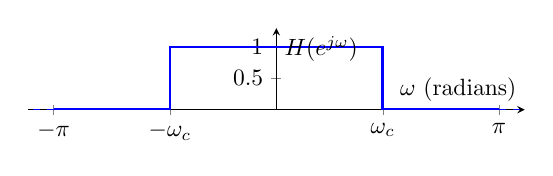
\begin{tikzpicture}[scale=0.85]
    \begin{axis}[
        width=9cm, height=2.8cm,
        xlabel={$\omega$ (radians)},
        ylabel={$H(e^{j\omega})$},
        xmin=-3.5, xmax=3.5,
        ymin=0, ymax=1.3,
        axis lines=middle,
        xtick={-3.14,-1.5,0,1.5,3.14},
        xticklabels={$-\pi$,$-\omega_c$,$0$,$\omega_c$,$\pi$}
    ]
    \addplot[blue, very thick] coordinates {(-3.14,0) (-1.5,0) (-1.5,1) (1.5,1) (1.5,0) (3.14,0)};
    \draw[blue, dashed, thick] (axis cs:3.14,0) -- (axis cs:4.64,0) -- (axis cs:4.64,1);
    \draw[blue, dashed, thick] (axis cs:-3.14,0) -- (axis cs:-4.64,0) -- (axis cs:-4.64,1);
    \end{axis}
\end{tikzpicture}
\end{center}

\textbf{Continuous-Time Frequency Response $H_c(j\Omega)$}:
\begin{center}
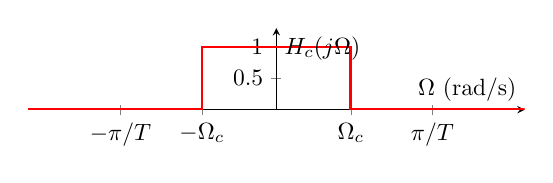
\begin{tikzpicture}[scale=0.85]
    \begin{axis}[
        width=9cm, height=2.8cm,
        xlabel={$\Omega$ (rad/s)},
        ylabel={$H_c(j\Omega)$},
        xmin=-5, xmax=5,
        ymin=0, ymax=1.3,
        axis lines=middle,
        xtick={-3.14,-1.5,0,1.5,3.14},
        xticklabels={$-\pi/T$,$-\Omega_c$,$0$,$\Omega_c$,$\pi/T$}
    ]
    \addplot[red, very thick] coordinates {(-5,0) (-3.14,0) (-1.5,0) (-1.5,1) (1.5,1) (1.5,0) (3.14,0) (5,0)};
    \end{axis}
\end{tikzpicture}
\end{center}

\textbf{Relationship}: $H_c(j\Omega) = H(e^{j\Omega T})$ for $|\Omega| < \pi/T$
\end{frame}

\section{Example: Noninteger Delay}

\begin{frame}{Example: Noninteger Delay System}
\textbf{Discrete-Time Frequency Response}:
\[
H(e^{j\omega}) = e^{-j\omega\Delta}, \quad |\omega| < \pi
\]

\vspace{0.3cm}
\textbf{Case 1 - Integer Delay} ($\Delta = n_0$, integer):
\[
y[n] = x[n - n_0]
\]
Straightforward interpretation: shift sequence by $n_0$ samples

\vspace{0.3cm}
\textbf{Case 2 - Noninteger Delay} ($\Delta$ not integer):
\begin{itemize}
    \item Expression $y[n] = x[n - \Delta]$ has no direct meaning
    \item Cannot shift discrete sequence by fractional samples
    \item Need continuous-time interpretation
\end{itemize}
\end{frame}

\begin{frame}{Continuous-Time Interpretation}
\textbf{Apply Design Relationship}:
\[
H_c(j\Omega) = H(e^{j\Omega T}) = e^{-j\Omega \Delta T}
\]

\vspace{0.3cm}
% \textbf{Recognition}: 
We recognize this is an ideal time delay
\[
y_c(t) = x_c(t - \Delta T)
\]

\vspace{0.3cm}
\textbf{Physical Interpretation}:
\begin{enumerate}
    \item Start with discrete sequence $x[n]$
    \item Reconstruct bandlimited $x_c(t)$ via D/C converter
    \item Delay $x_c(t)$ by $\Delta T$ seconds
    \item Sample delayed signal to get $y[n] = y_c(nT)$
\end{enumerate}

\vspace{0.3cm}
Therefore the noninteger delay operates on the \textbf{interpolated} continuous signal
\end{frame}

\begin{frame}{Noninteger Delay: Time Domain Visualization}
\textbf{Example}: $\Delta = 0.5$ (half-sample delay)

\begin{center}
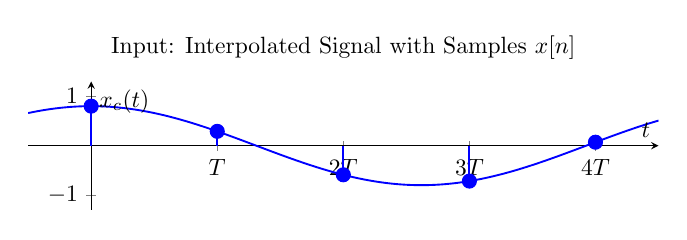
\begin{tikzpicture}[scale=0.85]
    \begin{axis}[
        width=11cm, height=3.5cm,
        xlabel={$t$},
        ylabel={$x_c(t)$},
        xmin=-0.5, xmax=4.5,
        ymin=-1.3, ymax=1.3,
        axis lines=middle,
        xtick={0,1,2,3,4},
        xticklabels={$0$,$T$,$2T$,$3T$,$4T$},
        title={Input: Interpolated Signal with Samples $x[n]$}
    ]
    % Interpolated continuous signal
    \addplot[blue, thick, domain=-0.5:4.5, samples=200] {0.8*cos(deg(1.2*x))};
    % Sample points (markers)
    \addplot[only marks, blue, mark=*, mark size=3pt] coordinates {
        (0,{0.8*cos(0)}) (1,{0.8*cos(deg(1.2))}) (2,{0.8*cos(deg(2.4))}) 
        (3,{0.8*cos(deg(3.6))}) (4,{0.8*cos(deg(4.8))})
    };
    % Stems using ycomb
    \addplot+[blue, ycomb, mark=none, thick] coordinates {
        (0,{0.8*cos(0)}) (1,{0.8*cos(deg(1.2))}) (2,{0.8*cos(deg(2.4))}) 
        (3,{0.8*cos(deg(3.6))}) (4,{0.8*cos(deg(4.8))})
    };
    \end{axis}
\end{tikzpicture}
\end{center}

\begin{center}
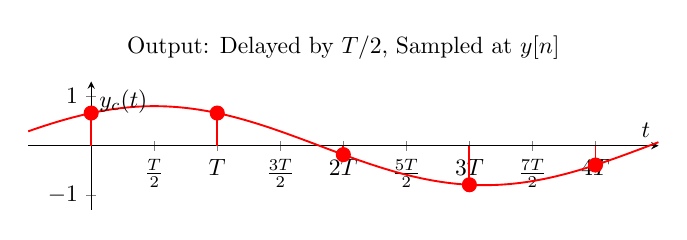
\begin{tikzpicture}[scale=0.85]
    \begin{axis}[
        width=11cm, height=3.5cm,
        xlabel={$t$},
        ylabel={$y_c(t)$},
        xmin=-0.5, xmax=4.5,
        ymin=-1.3, ymax=1.3,
        axis lines=middle,
        % show half-ticks but label the integer ticks as multiples of T
        xtick={0,0.5,1,1.5,2,2.5,3,3.5,4},
        xticklabels={$0$,$\frac{T}{2}$,$T$,$\frac{3T}{2}$,$2T$,$\frac{5T}{2}$,$3T$,$\frac{7T}{2}$,$4T$},
        title={Output: Delayed by $T/2$, Sampled at $y[n]$}
    ]
    % Delayed interpolated signal
    \addplot[red, thick, domain=-0.5:4.5, samples=200] {0.8*cos(deg(1.2*(x-0.5)))};
    % Sample points at integer times (shifted pattern)
    \addplot[only marks, red, mark=*, mark size=3pt] coordinates {
        (0,{0.8*cos(deg(-0.6))}) (1,{0.8*cos(deg(0.6))}) (2,{0.8*cos(deg(1.8))}) 
        (3,{0.8*cos(deg(3.0))}) (4,{0.8*cos(deg(4.2))})
    };
    % Stems using ycomb
    \addplot+[red, ycomb, mark=none, thick] coordinates {
        (0,{0.8*cos(deg(-0.6))}) (1,{0.8*cos(deg(0.6))}) (2,{0.8*cos(deg(1.8))}) 
        (3,{0.8*cos(deg(3.0))}) (4,{0.8*cos(deg(4.2))})
    };
    \end{axis}
\end{tikzpicture}
\end{center}
\end{frame}

\section{Example: Moving Average}

\begin{frame}{Example: Moving-Average System}
\textbf{General $(M+1)$-Point Moving Average}:
\[
y[n] = \frac{1}{M+1}\sum_{k=0}^{M}x[n-k]
\]

\vspace{0.3cm}
\textbf{Frequency Response} (from DTFT Lecture):
\[
H(e^{j\omega}) = \frac{1}{M+1}\frac{\sin[\omega(M+1)/2]}{\sin(\omega/2)}e^{-j\omega M/2}
\]

\vspace{0.3cm}
\textbf{Decomposition}:
\begin{center}
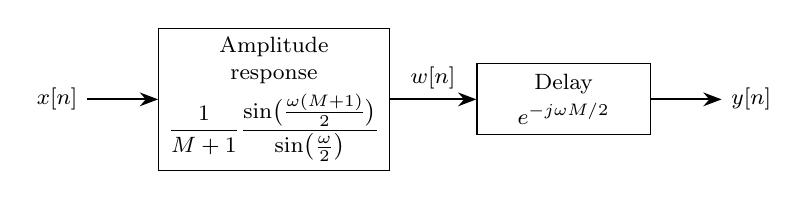
\begin{tikzpicture}[>=Stealth, node distance=1cm, auto, every node/.style={font=\footnotesize}]
  % compact, consistent block style
  \tikzset{block/.style={draw, minimum width=2.2cm, minimum height=0.9cm, align=center}}

  % nodes and layout
  \node (xn) {$x[n]$};
  \node[block, right=0.9cm of xn] (amp) {Amplitude\\response\\[3pt] $\displaystyle \frac{1}{M+1}\frac{\sin\!\big(\tfrac{\omega(M+1)}{2}\big)}{\sin\!\big(\tfrac{\omega}{2}\big)}$};
  \node[block, right=1.1cm of amp] (delay) {Delay\\[3pt] $\displaystyle e^{-j\omega M/2}$};
  \node (yn) [right=0.9cm of delay] {$y[n]$};

  % arrows and the intermediate discrete signal label w[n]
  \draw[->, thick] (xn.east) -- (amp.west);
  \draw[->, thick] (amp.east) -- (delay.west) node[midway, above] {$w[n]$};
  \draw[->, thick] (delay.east) -- (yn.west);
\end{tikzpicture}
\end{center}
\end{frame}

\begin{frame}{Moving Average: Integer vs. Noninteger Delay}
\textbf{Case 1 - Odd Number of Points} ($M$ even):

Example: $M = 4$ (5-point average)
\[
\text{Delay} = \frac{M}{2} = 2 \text{ samples (integer)}
\]
\[
y[n] = w[n - 2]
\]
Simple interpretation: 2-sample shift

\vspace{0.3cm}
\textbf{Case 2 - Even Number of Points} ($M$ odd):

Example: $M = 5$ (6-point average)
\[
\text{Delay} = \frac{M}{2} = 2.5 \text{ samples (noninteger)}
\]

Must use continuous-time interpretation:
\begin{itemize}
    \item Bandlimited interpolation of $w[n]$
    \item Continuous delay of $MT/2 = 2.5T$ seconds
    \item Resampling to get $y[n]$
\end{itemize}
\end{frame}


\begin{frame}{Moving Average: Numerical Example}
\textbf{Input}: $x[n] = \cos(0.25\pi n)$

\textbf{System}: 6-point moving average ($M = 5$)

\vspace{0.3cm}
\textbf{Frequency Response at Input Frequency}:
\[
H(e^{j0.25\pi}) = \frac{1}{6}\frac{\sin[3(0.25\pi)]}{\sin(0.125\pi)}e^{-j(0.25\pi)(2.5)}
\]

Calculate magnitude:
\[
|H(e^{j0.25\pi})| = \frac{1}{6}\frac{\sin(0.75\pi)}{\sin(0.125\pi)} \approx 0.308
\]

Calculate phase:
\[
\angle H(e^{j0.25\pi}) = -0.25\pi \times 2.5 = -0.625\pi
\]
\end{frame}

\begin{frame}{Moving Average: Visualization}
\small % reduce overall text size so plots + text fit vertically
\textbf{Input Signal}: $x[n] = \cos(0.25\pi n)$
\begin{center}
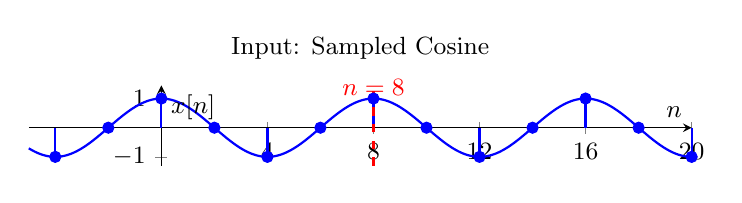
\begin{tikzpicture}
    \begin{axis}[
        width=10cm, height=2.6cm,    % plot size tuned to fit frame
        xlabel={$n$},
        ylabel={$x[n]$},
        xmin=-5, xmax=20,
        ymin=-1.3, ymax=1.45,        % extended top margin so vertical line and label are visible
        axis lines=middle,
        xtick={0,4,8,12,16,20},
        title={Input: Sampled Cosine},
        title style={font=\small},
        label style={font=\small},
        tick label style={font=\small},
        clip=false,                  % don't clip annotations outside the axis box
        enlarge y limits=false
    ]
    % Continuous interpolation
    \addplot[blue, thick, domain=-5:20, samples=300] {cos(deg(0.25*pi*x))};
    % Sample points at the chosen integer positions
    \addplot[only marks, blue, mark=*, mark size=2pt, samples at={-4,-2,0,2,4,6,8,10,12,14,16,18,20}] {cos(deg(0.25*pi*x))};
    % Stems using ycomb at the same sample positions
    \addplot+[blue, ycomb, mark=none, thick, samples at={-4,-2,0,2,4,6,8,10,12,14,16,18,20}] {cos(deg(0.25*pi*x))};
    % Vertical dashed line marking the input peak at n=8 (now inside axis extent)
    \addplot[red, dashed, thick] coordinates {(8,-1.3) (8,1.3)};
    % Label slightly above the top of the plotted curve (uses clip=false so it is visible)
    \node[red, font=\small] at (axis cs:8,1.38) {$n=8$};
    \end{axis}
\end{tikzpicture}
\end{center}

\textbf{Output Signal}: $y[n] = 0.308\cos[0.25\pi(n-2.5)]$
\begin{center}
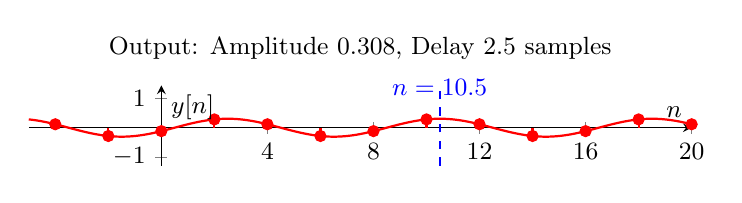
\begin{tikzpicture}
    \begin{axis}[
        width=10cm, height=2.6cm,    % match the first plot's reduced height
        xlabel={$n$},
        ylabel={$y[n]$},
        xmin=-5, xmax=20,
        ymin=-1.3, ymax=1.45,        % extended top margin so vertical line and label are visible
        axis lines=middle,
        xtick={0,4,8,12,16,20},
        title={Output: Amplitude 0.308, Delay 2.5 samples},
        title style={font=\small},
        label style={font=\small},
        tick label style={font=\small},
        clip=false,                  % ensure annotations outside axis aren't clipped
        enlarge y limits=false
    ]
    % Continuous interpolation (delayed and scaled)
    \addplot[red, thick, domain=-5:20, samples=300] {0.308*cos(deg(0.25*pi*(x-2.5)))};
    % Sample points at the same integer positions
    \addplot[only marks, red, mark=*, mark size=2pt, samples at={-4,-2,0,2,4,6,8,10,12,14,16,18,20}] {0.308*cos(deg(0.25*pi*(x-2.5)))};
    % Stems using ycomb
    \addplot+[red, ycomb, mark=none, thick, samples at={-4,-2,0,2,4,6,8,10,12,14,16,18,20}] {0.308*cos(deg(0.25*pi*(x-2.5)))};
    % Vertical dashed line marking the output peak at n=10.5 (inside axis extent)
    \addplot[blue, dashed, thick] coordinates {(10.5,-1.3) (10.5,1.3)};
    \node[blue, font=\small] at (axis cs:10.5,1.38) {$n=10.5$};
    \end{axis}
\end{tikzpicture}
\end{center}
\end{frame}



\section{Summary}

\begin{frame}{Summary: Concepts}
\textbf{System Architecture}:
\[
x[n] \xrightarrow{\text{D/C}} x_c(t) \xrightarrow{H_c(j\Omega)} y_c(t) \xrightarrow{\text{C/D}} y[n]
\]

\vspace{0.3cm}
\textbf{Fundamental Relationships}:
\[
H(e^{j\omega}) = H_c\left(j\frac{\omega}{T}\right) \quad \Leftrightarrow \quad H_c(j\Omega) = H(e^{j\Omega T})
\]

\vspace{0.3cm}
\textbf{Limitations}:
\begin{itemize}
    \item Not typically used for actual implementation
    \item Requires bandlimited signals for exact analysis
    \item Mainly a conceptual/analytical tool
\end{itemize}

\end{frame}


\begin{frame}{Summary: Mathematical Framework}
\textbf{Time Domain}:
\[
x_c(t) = \sum_{n=-\infty}^{\infty}x[n]\frac{\sin[\pi(t-nT)/T]}{\pi(t-nT)/T}
\]

\[
h[n] = \frac{\sin[\pi(n-\Delta)]}{\pi(n-\Delta)} \text{ for delay } \Delta
\]

\vspace{0.3cm}
\textbf{Frequency Domain}:
\[
X_c(j\Omega) = TX(e^{j\Omega T}), \quad Y_c(j\Omega) = H_c(j\Omega)X_c(j\Omega)
\]

\[
Y(e^{j\omega}) = \frac{1}{T}Y_c\left(j\frac{\omega}{T}\right) = H_c\left(j\frac{\omega}{T}\right)X(e^{j\omega})
\]

\vspace{0.3cm}
\textbf{Design Equation}:
\[
\boxed{H_c(j\Omega) = H(e^{j\Omega T}), \quad |\Omega| < \pi/T}
\]
\end{frame}

\end{document}